\chapter{A motivation for studying fluid-structure interaction}
Fluid-structure interaction(FSI) forms the basis of many physical phenomena in nature. A fish swimming upstream,
generating thrust from the surrounding fluid by wave-like movements of its fin and body. Or a tree, bedning back and fourth due to strong winds of a storm passing by. FSI has also proved to be essential for design development and performance optimalizastion of many engineering applications. Applications are, but not limited to biomedical computations such as heart valves and aneurisms \cite{Torii2008, Vierendeels2007} inflation of parachutes \cite{Stein2001}, underwater explosions \cite{Kim2008} and wind turbines \cite{Hsu2012}. Within aeronautics, FSI have proven to be crucial for advances within flight characteristics and fuel economy. Due to a wide range of wing materials and flow profiles to be studied, FSI have made testing of proposed models possible. One contribution is the development of winglets. \\

\begin{wrapfigure}{r}{5cm}
%\centering
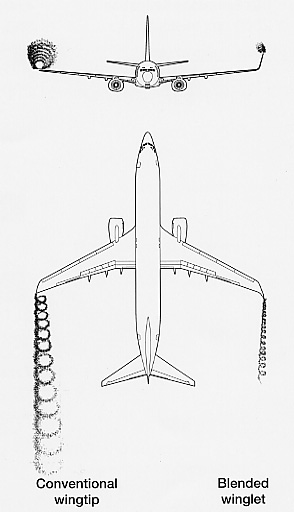
\includegraphics[scale=0.5]{./Fig/winglet.png}
  \caption{A comparison of shedding vortices from conventional wingtip, versious a winglet.}
  \vspace{-120pt} 
\end{wrapfigure}
A winglet is a near vertical tip replacement for a conventional wingtip of an aircraft, which have reduced drag induced by wingtip vortices during flight. As a result, the overall fuel consumption of long-distance flights have been reduced by $\sim 5 \%$, which is why winglets can be observed within many airliners today. Another consequence of installing wingelts is the reduction of wingtip vortices, which in turn reduces trailing turbulence behind the aircraft.  The trailing turbulence can intervene with flight controls of aircraft passing through it, making  wingles an important safety feature for flight traffic.



\newpage

Fluid-structure interaction is advantageous in comparison with full-scale experiments. Constructing material models and conducting flow experiments together, can be both expensive and time-consuming. Development of accurate and efficient solvers for FSI is therefore of great importance for further research. In this thesis, I present a monolithic FSI solver based on the arbitary Langrangian-Eulerien(ALE) method \cite{Donea2004}, where the equations of fluid and structure are solved simultaneous by Newton's method. In general, the ALE method is favorable for connecting the physics of fluid and structure, which are fundamentally formulated different. However, a monolithic ALE approach lacks computational efficiency due to the overall size of the problem, and due to mesh degeneration by the structure deformation. It is my intention to investigate these limitations, and to give a comparison of methods considered to improve computational efficiency. \\

The primary goals of this thesis are:

\begin{itemize}
\item Formulate a finite element variation formulation for a monolithic ALE fluid-structure interaction problem.
\item Construct a finite element solver for the full FSI problem, by Newton's method.
\item Compare different methods to avoid mesh degeneration.
\item Improve computational efficiency for the FSI solver, for a chosen validation benchmark.
\end{itemize}